\documentclass[12pt,a4paper]{article}
\usepackage[utf8]{inputenc}
\usepackage[german]{babel}
\usepackage[T1]{fontenc}
\usepackage{amsmath}
\usepackage{amsfonts}
\usepackage{amssymb}
\usepackage{graphicx}
\usepackage[left=2.5cm,right=2.5cm,top=2cm,bottom=2cm]{geometry}
\usepackage{float}
\author{Gruppe C14 \\ Julián Häck, Martin Koytek, Lars Wenning, Erik Zimmermann}
\begin{document}
\section{Residuen}
Bei der Korrektur des Residuenplots für die Lineare Regression der Hauptmessung, wurde die Fehlerrechnung durch:
\begin{equation}
\sigma_R=\sqrt{\sigma_{\ln(p)}^2+(a\cdot \sigma_{\frac{1}{T}})^2}
\end{equation}
(mit der Steigung der Linearen Regression a) ersetzt. 
\begin{figure}[H]
\centering
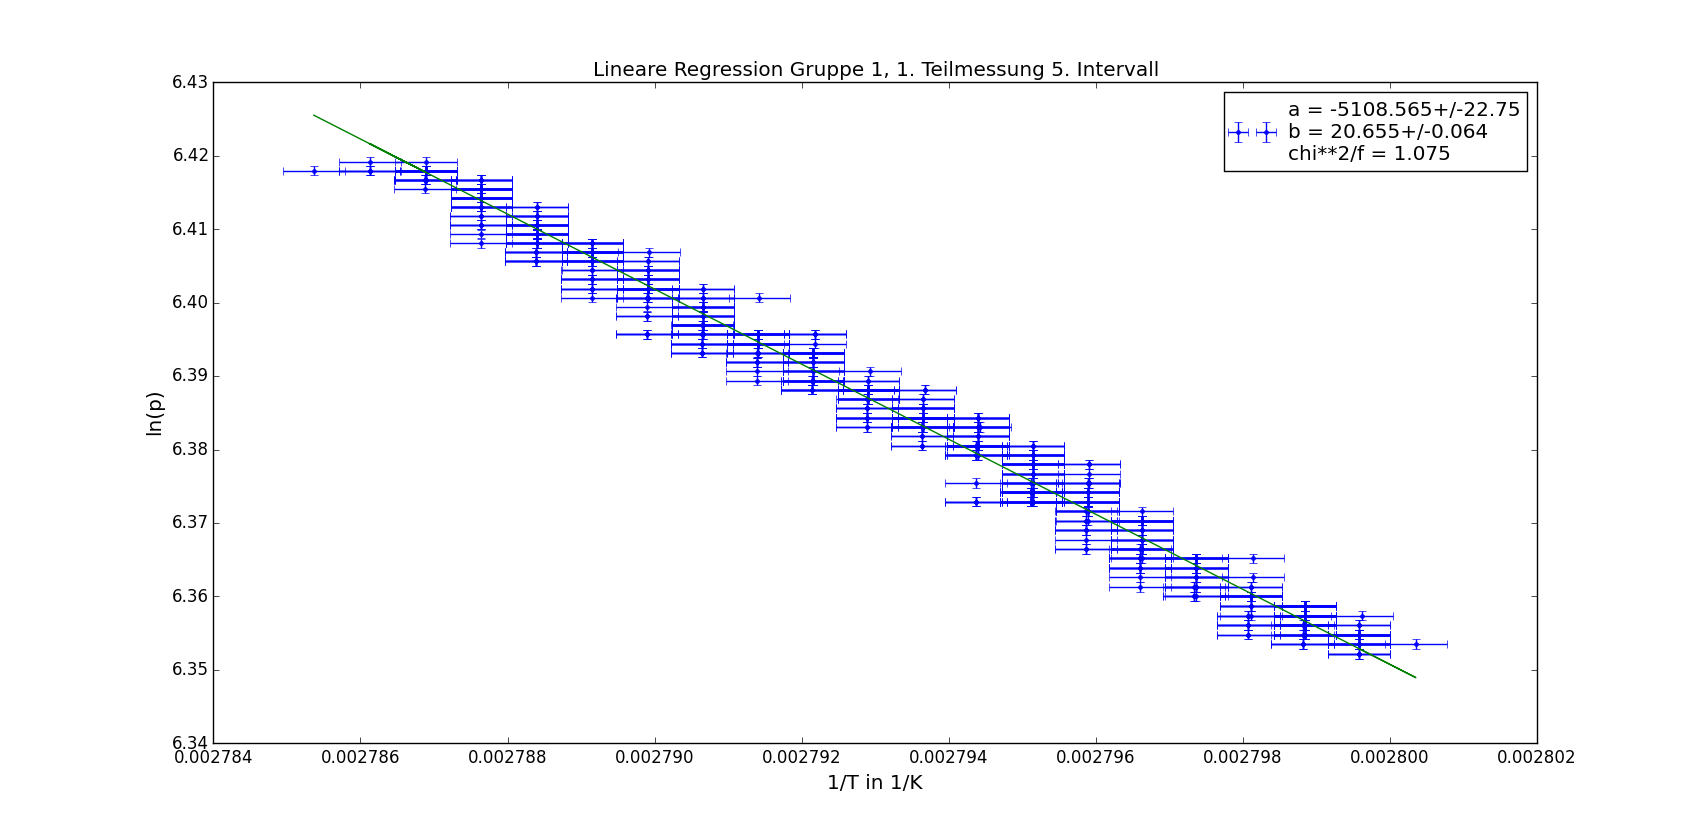
\includegraphics[scale=0.4]{G1_Intervall5_LinReg.png}
\caption{Beispiel Lineare Regression Gruppe 1}
\end{figure}
\begin{figure}[H]
\centering
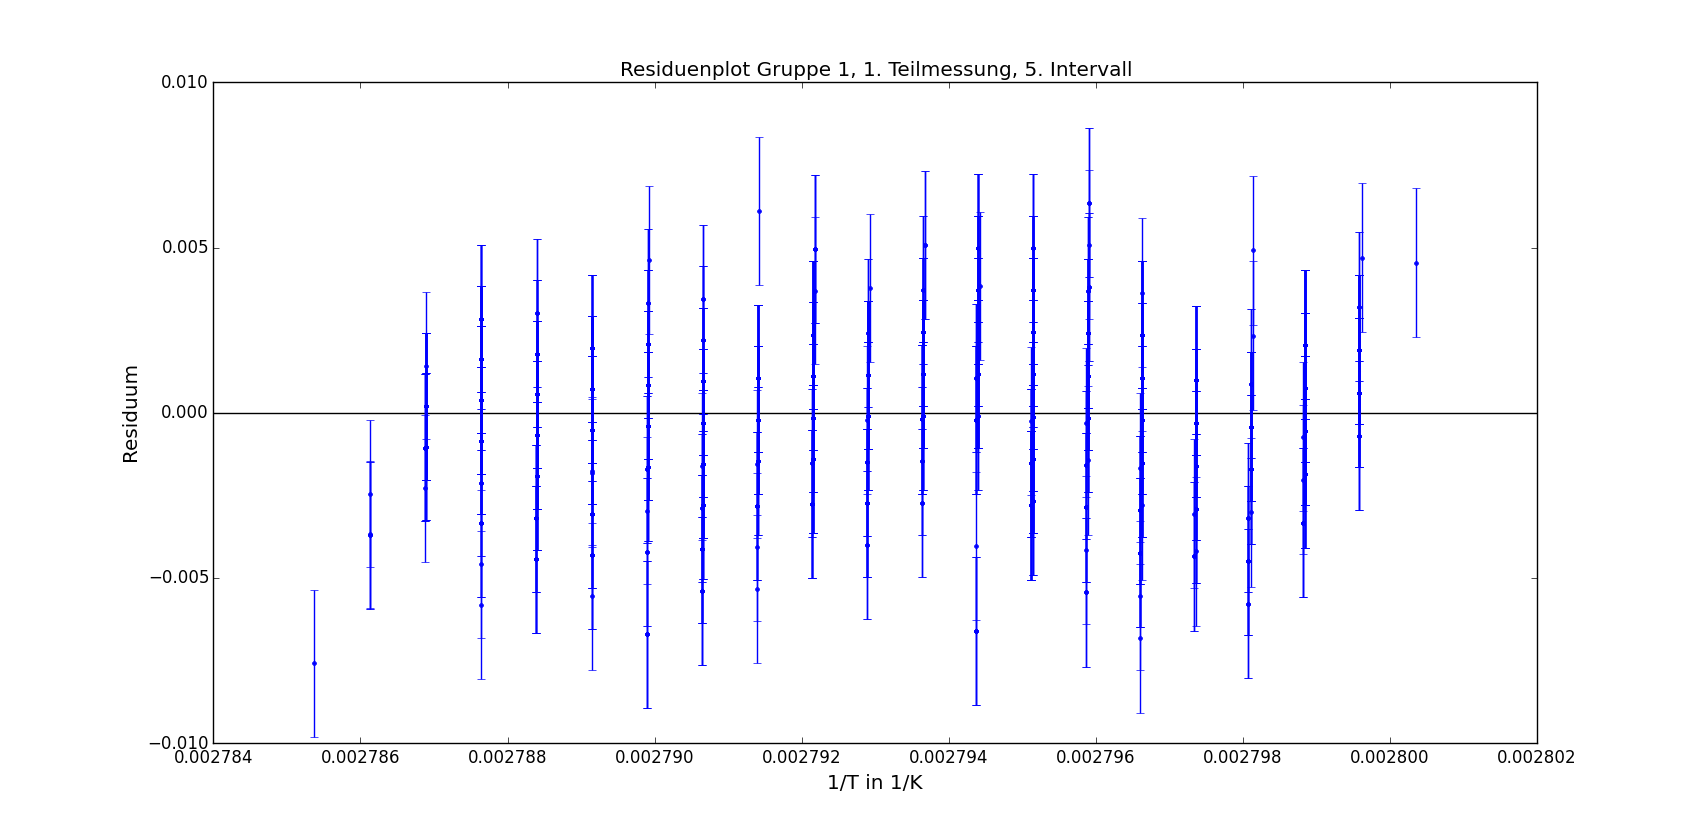
\includegraphics[scale=0.4]{G1_Intervall5_Residuen.png}
\caption{Beispiel Residuen Gruppe 1}
\end{figure}
\begin{figure}[H]
\centering
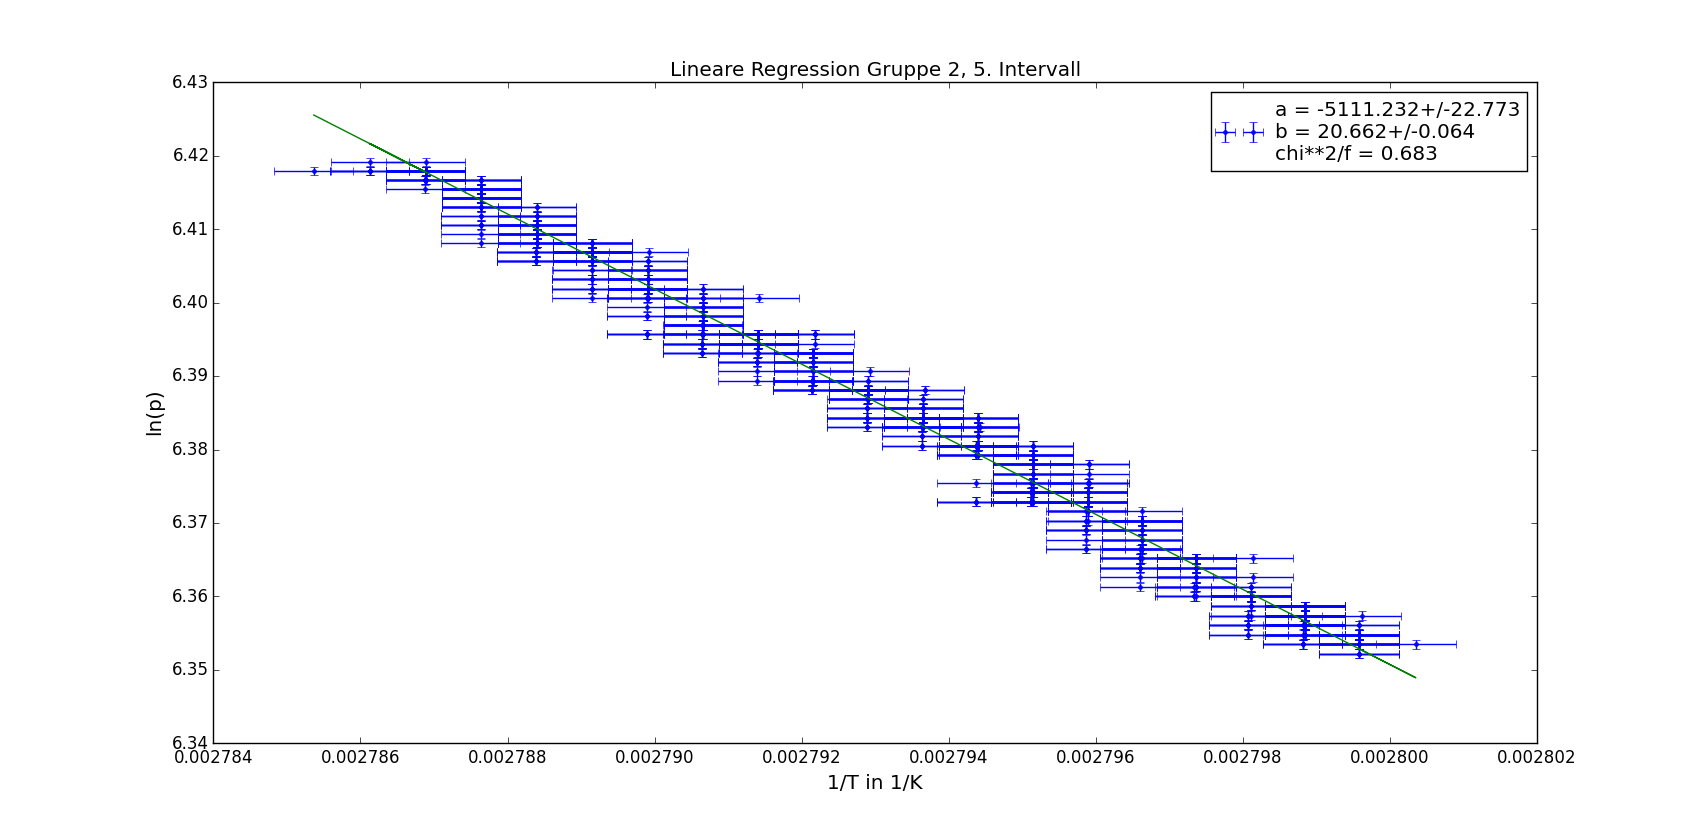
\includegraphics[scale=0.4]{G2_Intervall5_LinReg.png}
\caption{Beispiel Lineare Regression Gruppe 2}
\end{figure}
\begin{figure}[H]
\centering
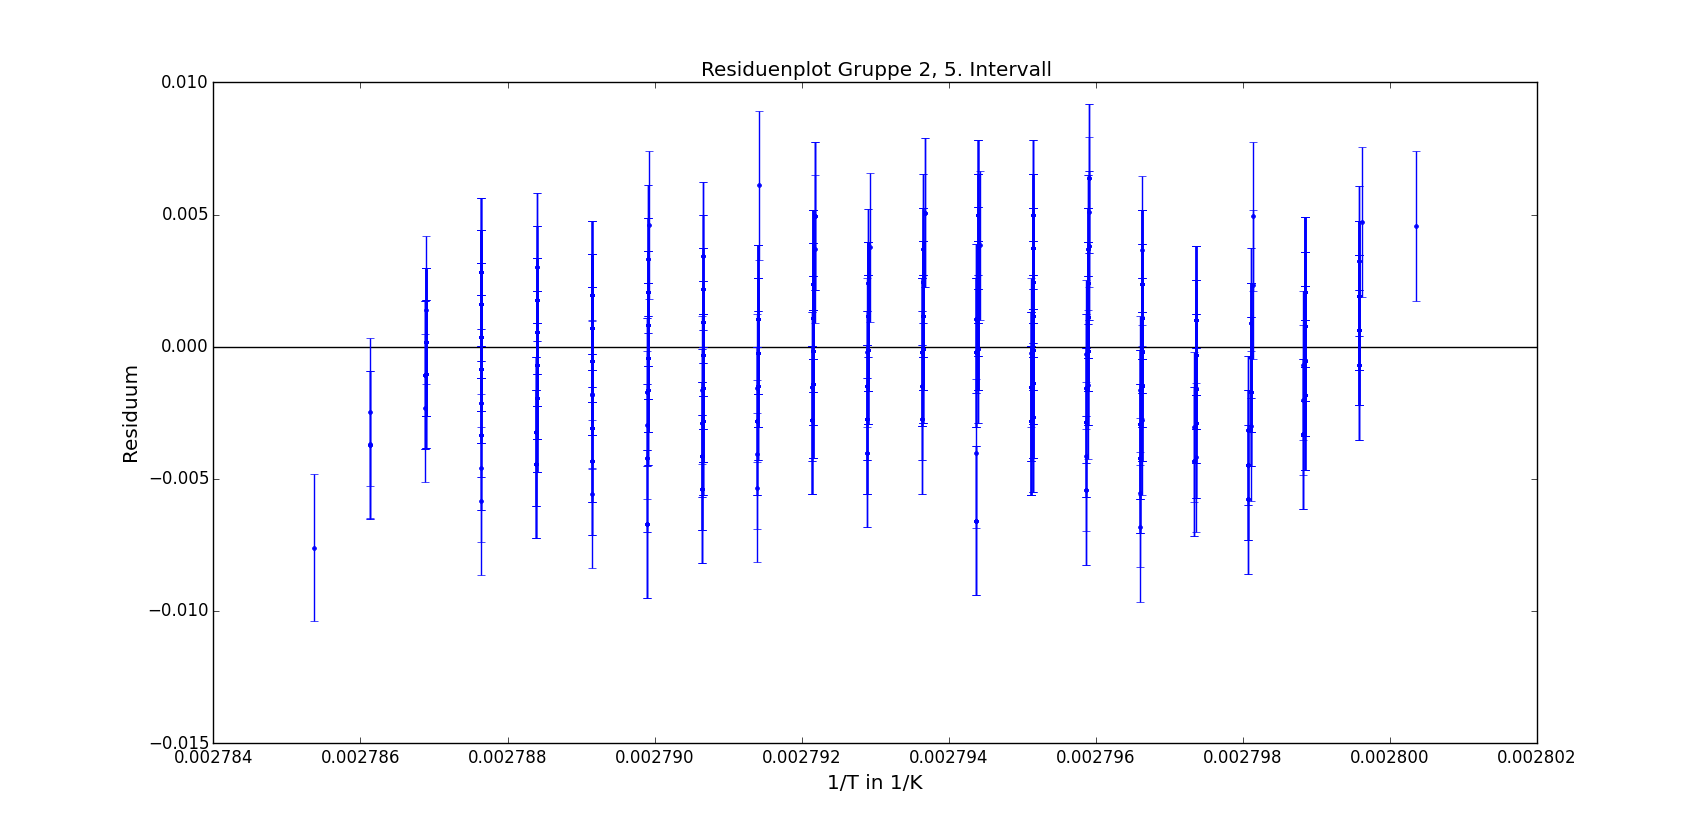
\includegraphics[scale=0.4]{G2_Intervall5_Residuen.png}
\caption{Beispiel Residuen Gruppe 2}
\end{figure}

\end{document}